\documentclass{article}


\usepackage{arxiv}

\usepackage[utf8]{inputenc} % allow utf-8 input
\usepackage[T1]{fontenc}    % use 8-bit T1 fonts
\usepackage{hyperref}       % hyperlinks
\usepackage{url}            % simple URL typesetting
\usepackage{booktabs}       % professional-quality tables
\usepackage{amsfonts}       % blackboard math symbols
\usepackage{nicefrac}       % compact symbols for 1/2, etc.
\usepackage{microtype}      % microtypography
\usepackage{lipsum}

\usepackage{graphicx}
\usepackage{caption}
\usepackage{subcaption}

\title{Concrete Dropout: \\Experiments replication and Extensions}


\author{
  Valerii Likhosherstov \\
  Statistical Learning Theory Joint Master Program \\
  Skolkovo Institute of Science and Technology\\
  \texttt{Valerii.Likhosherstov@skoltech.ru} \\
  %% examples of more authors
   \And
 Alfredo de la Fuente \\
 Statistical Learning Theory Joint Master Program\\
 Skolkovo Institute of Science and Technology\\
  \texttt{Alfredo.Delafuente@skoltech.ru} \\
  %% \AND
  %% Coauthor \\
  %% Affiliation \\
  %% Address \\
  %% \texttt{email} \\
  %% \And
  %% Coauthor \\
  %% Affiliation \\
  %% Address \\
  %% \texttt{email} \\
  %% \And
  %% Coauthor \\
  %% Affiliation \\
  %% Address \\
  %% \texttt{email} \\
}

\begin{document}
\maketitle

\begin{abstract}
In this project we reproduce the results of the paper "Concrete Dropout" by Gal et al. (\cite{concrete}). We go further by extending the range of experiments and implementing the Concrete Dropout for Natural Language Processing tasks. Furthermore, we provide an efficient implementation of a fully connected, spatial convolution and LSTM Concrete Dropout layers.
\end{abstract}


% keywords can be removed
\keywords{bayesian deep learning, concrete dropout, model uncertainty}


\section{Background}

Imposing a prior over the weights of a neural network and adopting a fully Bayesian inference in this rich class of estimators provides multiple advantages. First, integrating model parameters out through the MC-estimate of the integral during prediction results in a better performance \cite{bconvnn} compared to using a point MAP estimate of weights, as it happens in vanilla-dropout \cite{dropout}. Second, MC-estimates of predictions' second moments give the information about model's uncertainty on the given example \cite{uncertainty}. Uncertainty gives a tool for human-guided model fitting, when the train set can be augmented with new examples of uncertain objects. One valuable area of application for uncertainty estimates (both epistemic and predictive) is Reinforcement Learning, where grid searching is clearly unfeasible and dropout has to be adapted dynamically, considering that the agent is expected to reduces its uncertainty as the data increases for a good model calibration. In addition, a remarkable feature of dropout's Bayesian interpretation is that with certain priors and variational approximation family, it results in sparse weight matrices \cite{sparse}, enabling more flexible and regularized models. \\

Originally, the Bayesian interpretation was only introduced for Gaussian dropout \cite{welling}, where the re-parametrization trick (or pathwise derivative) allows to obtain unbiased gradient estimates with low variance. Unfortunately, pathwise derivative is not available for discrete random variables - a case of Bernoulli dropout. As an alternative solution, the log-derivative trick and REINFORCE scheme \cite{Williams1992} suffers from high variance in stochastic gradients. For these reasons, a continuous relaxation of discrete random variables was elaborated to solve this problem - using the Gumbel-Softmax distribution \cite{gumbel}, which converges to discrete distribution at high temperatures and is compatible with the reparametrization trick. In \cite{gumbel}, authors exclusively employ Gumbel-Softmax to model discrete hidden states. In \cite{concrete} they use a special case of Gumbel-Softmax with two possible states (Concrete distribution) to approximate Bernoulli dropout during training. Also, a correct choice of prior results in a tractable KL-divergence between prior and variational approximation, which simplifies computations.

\section{Concrete Dropout}
\label{sec:headings}
In order to overcome the computationally intensive task of grid searching over the dropout probability space, specially in scenarios of dealing with complex models with large datasets and under continuous learning settings where the epistemic uncertainty should decrease as more data is collected; the authors suggest to incorporate the dropout rate in the loss function and thus optimize directly it using gradient methods. \\

\subsection{Derivation of the Loss function}
Following the variational interpretation of dropout \cite{Gal2016Uncertainty}, we can see it as an approximating distribution $q_\theta(\omega)$ to the posterior in a Bayesian neural network with a set of random weight matrices $ \omega = \left[ W_l \right]_{l=1}^L$  with $L$ layers and $\theta$ being the set of variational parameters. Then, the optimization objective can be written as follows, 

\begin{equation}\label{eq1}
    \hat{\mathcal{L}}_{MC} (\theta) = -\frac{1}{M} \sum_{i\in S} \log p\left( y_i\vert f^{\omega} ( x_i ) \right) + \frac{1}{N} \mathbb{KL} \left( q_\theta(\omega) \Vert p(\omega) \right)
\end{equation}

where $N$ is the number of data points, $S$ a random set of $M$ data points, $f^\omega(x_i)$ the neural network's output on input $x_i$ with parameters $\omega$ and $p(y_i\vert f^\omega (x_i) $ the model's likelihood (e.g. Gaussian with mean $f^\omega (x_i) $). The regularization term ensures that the approximate posterior $q_\theta(\omega)$ does not deviate too far from the prior distribution $p(\omega)$. The prior was chosen to be a discrete quantised Gaussian as described in the paper \cite{Gal2016Uncertainty}. We can assume that the set of variational parameters for t he dropout 

\begin{equation}\label{eq2}
    \mathbb{KL}\left( q_\theta(\omega) \Vert p(\omega) \right) = \sum_{l=1}^L \mathbb{KL}\left( q_{M_l} ( W_l \Vert p(W_l) \right) \propto \frac{l^2(1-p)}{2} \|M\|^2 - K \mathcal{H}(p).
\end{equation}

where $K$ is 

\subsubsection{Concrete Distribution}

One of the main restrictions, as previously mentioned,  relies on the evaluation of the derivative of the objective function with respected to the dropout rate $p$ for the loss optimization step.  The preferred estimator in the literature is  pathwise estimator, however we need to be able to express 

\begin{equation}\label{eq3}
    \bar{z} =  \textit{sigmoid} \left( \frac{1}{t} \dot \left( \log \frac{p}{1-p}  + \log \frac{u}{1-u}    \right)  \right) 
\end{equation}

where $u\sim \text{Unif}(0,1)$ and $t$ is the temperature variable 

\subsection{Concrete Dropout for LSTM Layer}

We give a simple extension to Concrete dropout for the case of recurrent layer - LSTM. Let's revise the definition of LSTM\footnote{https://pytorch.org/docs/stable/nn.html#torch.nn.LSTM}:
\[
\begin{split}\begin{array}{ll}
i_t = \sigma(W_{ii} x_t + b_{ii} + W_{hi} h_{(t-1)} + b_{hi}) \\
f_t = \sigma(W_{if} x_t + b_{if} + W_{hf} h_{(t-1)} + b_{hf}) \\
g_t = \tanh(W_{ig} x_t + b_{ig} + W_{hg} h_{(t-1)} + b_{hg}) \\
o_t = \sigma(W_{io} x_t + b_{io} + W_{ho} h_{(t-1)} + b_{ho}) \\
c_t = f_t c_{(t-1)} + i_t g_t \\
h_t = o_t \tanh(c_t)
\end{array}\end{split}
\]

When using dropout with LSTM, we usually put it before the layer (at least we did that in experiments). From LSTM's definition it's clear, that this is equivalent to zeroing out columns of $W_{ii}, W_{if} W_{ig}, W_{io}$. So we only induce prior for $W_{ii}, W_{if} W_{ig}, W_{io}$ and consequently, only these matrices should be used in weight regularizer of our ELBO objective. This concludes our derivation of Concrete dropout for LSTM.

\paragraph{Paragraph} 


\section{Experiments}
\label{sec:experiments}

We analyze and validate the performance of Concrete Dropout in a wide variety of tasks. 

\subsection{Regression Task - UCI Datasets}

In this experiment we employ Concrete dropout to solve a regression task for 3 datasets from UCI base\footnote{https://archive.ics.uci.edu/ml/datasets.html}: Boston Housing Dataset, KIN8NM robotic arm dinamics dataset and Wine Quality Dataset.

We utilize a neural network of 3 fully-connected layers, each with 50 hidden units and concrete dropout. This network predicts a mean value of normally distributed output for regression. We also train a single value of log-precision parameter $\log \tau$ of output's distribution, for which we impose a prior distribution $\text{Gamma}(0.1, 0.01)$ (consequently, we add prior's logarithm to our objective function). We use weight and dropout regularizer of $10^{-2}$ and $10^2$ respectively.

In \cite{concrete} they alternate between tuning $\tau$ and variational parameters - a so-called variational (MAP)-EM algorithm. When we replicated this setting, we have found out that dropout probabilities are hardly changing from their initial random values. Hence, we have added third pass through the data to this alternating scheme, where we only tune dropout probabilities.

In our experiments, we try to replicate a pattern of converged dropout probabilities, which is invariant to cross-validation splits. See Figure \ref{fig:uci} for results. We observe a well-distinguished dropout probabilities between first two and the last layer (Wine dataset). For KIN8NM, first two layers converge to low dropout probabilities with small variance, while the last layer exposes a higher variability over cross-validation splits. For Boston, we do not observe any stable pattern.

\subsection{MNIST}
We used the standard classification dataset MNIST \cite{lecun-mnisthandwrittendigit-2010} to assess the accuracy of Concrete dropout and it's relation with the training-set size, by applying it in a Multi-Layer Perceptron (MLP) arquitecture with $3$ hidden layers (with $512$ units) and ReLU activations.

After trained for $100$ epochs, our Concrete dropout achieves MNIST accuracy of $~98\%$  matching that of hand-tuned dropout. Figure \ref{fig:mnist_frac} shows a decreasing converged dropout probabilities as the size of data increases for each one of the MLP layers. 

\subsection{Computer Vision}

FC-DenseNet model \cite{densenet} shows state-of-the-art results in image segmentation task. We try to further improve the model by substituting each dropout layer in it with its concrete version.

In our experiments we use \textit{FC-DenseNet103} topology with 103 convolution layers inside. For it we use a spatial version of Concrete dropout, when the whole channels are "zeroed-out". We opt for weight regularizer of $10^{-8}$ and dropout regularizer of $10^0$. The model is trained for 100 epochs with RMSprop (learning rate - $10^{-4}$). We figured out, that starting from small random dropout probabilities ($0.01-0.05$) results in a better performance of the model.

We compare Concrete dropout with grid-searched dropout rate of $0.2$ (reported in \cite{densenet}). Figure \ref{fig:segcurve} reports average Intersection-over-Union score over 12 segmentation classes on training and validation set. Concrete dropout performed better on a validation set, even though training takes more time for it. If to encounter that dropout baseline required grid search, Concrete dropout appears to be more advantageous. On testing set, concrete dropout reached IoU of $0.414$ and $0.418$ with MC predictions against $0.401$ for dropout.

Figure \ref{fig:calib_ex} (a) shows calibration plots for each segmentation class. Concrete dropout with MC predictions is the closest to a diagonal. Strangely, if don't use MC for predicting, it results in worse-calibrated predictions then dropout in most cases. Figure \ref{fig:calib_ex} (b) illustrates predictions and uncertainties.

\subsection{Reinforcement Learning Task}

\subsection{Natural Language Processing}

In this subsection we go beyond the scope of \cite{concrete} and apply Concrete dropout to solve real-life tasks in Natural Language Processing. We comment the results from a user standpoint, i.e. like if a data scientist was trying to add Concrete dropout feature into his model.

\subsubsection{Grapheme to Phoneme}

We tackle the problem a grapheme-to-phoneme \footnote{https://www.kaggle.com/c/grapheme-to-phoneme}, where we have to predict English word's transcription. We applied the following architecture for our model: an encoder that consists of embedding size 100, then 3 LSTM layers with 100 hidden units and batch-norm and dropout before each. Next, we used average-pooling over encoder outputs, repeated it and put as an input to decoder - two layers of LSTM blocks same as in encoder, followed by linear layer and softmax. We trained our model for 100 epochs with RMSprop (learning rate - $10^{-3}$).

For dropout, we check performance of different probabilities on a validation set. For concrete dropout, we use weight regularizer of $10^{-4}$ and try different values of dropout regularizer. As a metric, we use average Hamming distance between ground truth and predicted word.

Figure \ref{fig:nlpcurves} presents learning curves for dropout and Concrete dropout. We find, that Concrete dropout performs slightly worse than dropout. We also see that Concrete dropout overfits - that happens because dropout probabilities converge to zero (Figure \ref{fig:nlpprobs}). All in all, we didn't manage to glue Concrete dropout with LSTM to obtain good results in this task.

\subsubsection{Sentiment Classification Task - SST dataset }

For this task we used the well-known Stanford Sentiment Treebank dataset  \cite{socher2013}\footnote{https://nlp.stanford.edu/sentiment/treebank.html} in its binary form. This dataset contains movie reviews which are annotated by positive or negative sentiment labels. Our proposed model is composed by one embedding layer of size $100$, one  LSTM layer with $256$ hidden units and followed by a fully connected layer to the binary output. 

We run the model with a fixed dropout rate of $0.5$ to compare it against the implemented ConcreteDropout version of the LSTM layer. We used batches of $64$ observations, weight regularizer $10^{-6}$ and dropout regularizer $2\times 10^{-5}$. 

The results after training for $20$ epochs with Adam optimizer we obtained are shown at $\ref{fig:sentiment}$. We can observe that our ConcreteDropout LSTM model was able to surpass the baseline model accuracy for the validation set by taking only a few more iterations to converge. This suggests that our model is able to tune dropout rate faster, while not risking predictive accuracy.  

\section{Conclusions and Remarks}
 
 In this research project, we were able to validate and demonstrate how tuning the dropout rate via concrete dropout can provide us an speed up in comparison with grid-searching. One drawback of this model reflects on the need to tune hyperparameters such as weight regularizer and dropout regularizer which can dramatically affect the model predictions. Although the original paper suggests some rule of thumbs, it is still unclear how to tune the values without using a grid-search approach. We should also mention as insight, that the dropout probabilities obtained for different layers follow the general knowledge about using smaller dropout for shallow layers in a neural network. Finally, based on our reproducibility results, we can conclude that the performance of the concrete dropout layer model is comparable with the one of the model with optimal dropout probability fixed, making it much faster than grid-search with exponential number of dropout combinations. 

\bibliographystyle{unsrt}
\bibliography{references}


\newpage
\section{Appendix}

In this section we display all relevant plots of results referenced in the experimental section.
\begin{figure}[!h]
\centering
\begin{subfigure}{.33\textwidth}
  \centering
  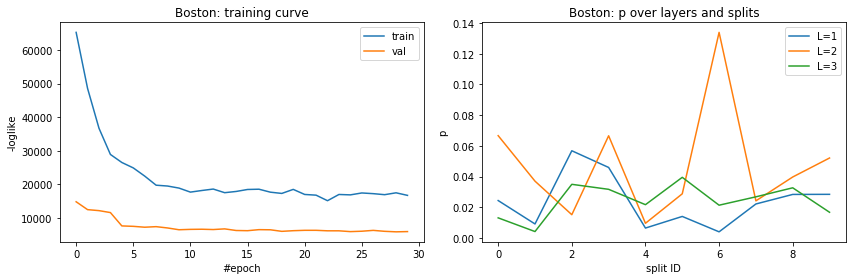
\includegraphics[width=\linewidth]{boston.png}
  \caption{Boston}
\end{subfigure}%
\begin{subfigure}{.33\textwidth}
  \centering
  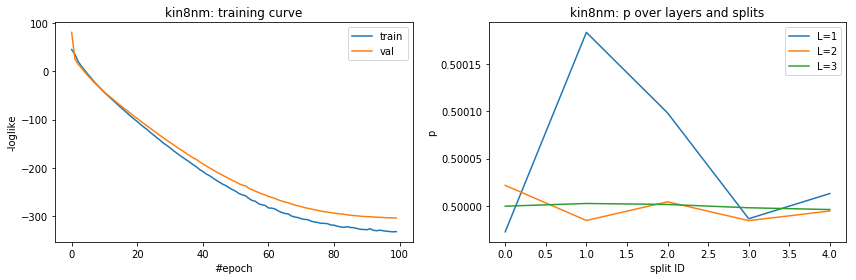
\includegraphics[width=\linewidth]{kin8nm.png}
  \caption{KIN8NM}
\end{subfigure}%
%\vskip\baselineskip
\begin{subfigure}{.33\textwidth}
  \centering
  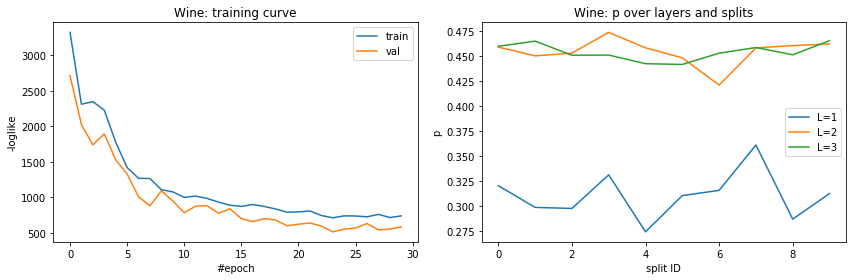
\includegraphics[width=\linewidth]{wine.png}
  \caption{Wine}
\end{subfigure}
\caption{UCI experiments. Best viewed on a computer screen.}
\label{fig:uci}
\end{figure}


\begin{figure}[!h]
\centering
\centering
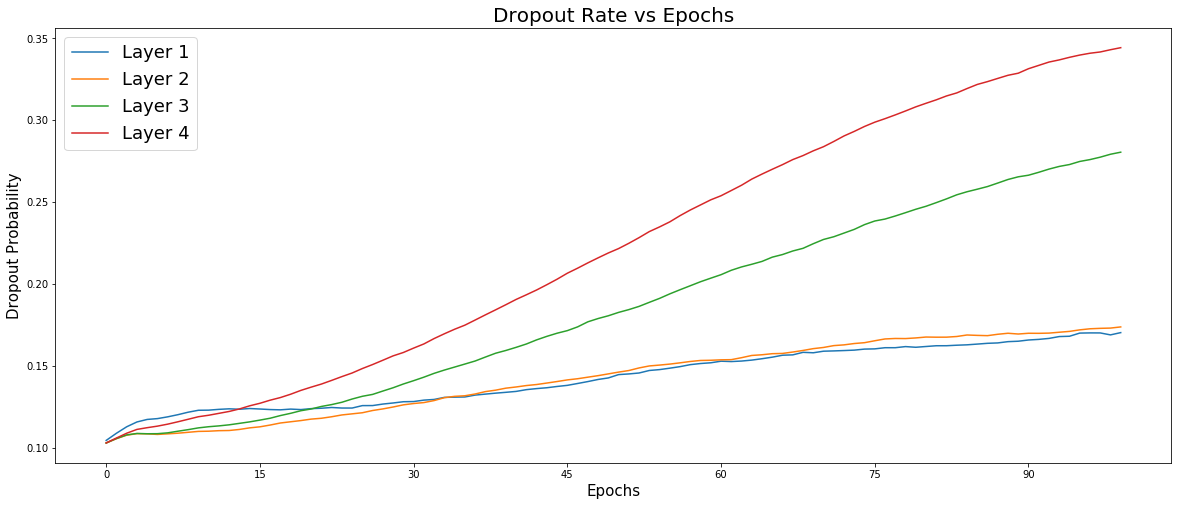
\includegraphics[width=0.5\linewidth]{dropout_convergence_100.png}
\caption{Convergence of Dropout Probabilities per Layer given different fractions of training set.}
\label{fig:mnist_frac}
\end{figure}


\begin{figure}[!h]
\centering
\centering
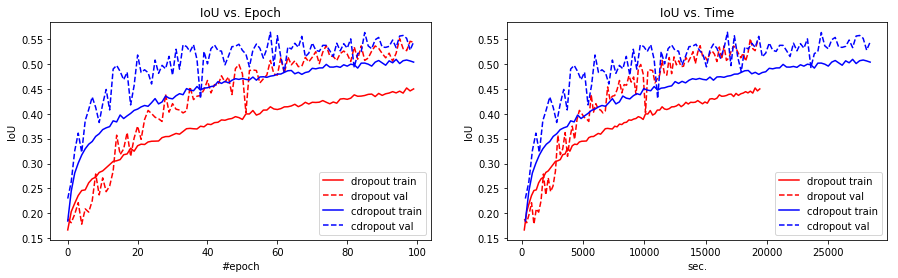
\includegraphics[width=0.7\linewidth]{time_iou_comparison.png}
\caption{Segmentation: learning curves.}
\label{fig:segcurve}
\end{figure}

\begin{figure}[!h]
\centering
\centering
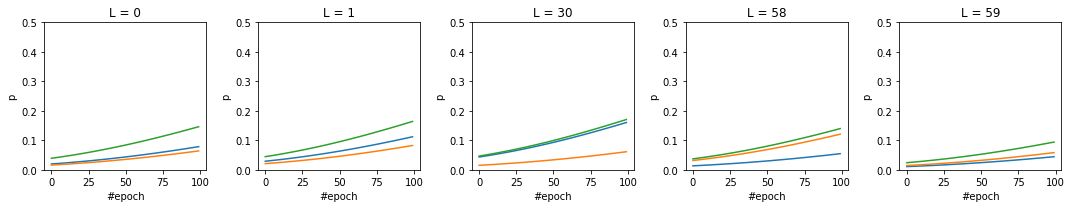
\includegraphics[width=\linewidth]{dropout_rate_convergence.png}
\caption{Segmentation: dropout rate convergence over layers and several data fits.}
\label{fig:segconv}
\end{figure}

\begin{figure}[!h]
\centering
\begin{subfigure}{.5\textwidth}
  \centering
  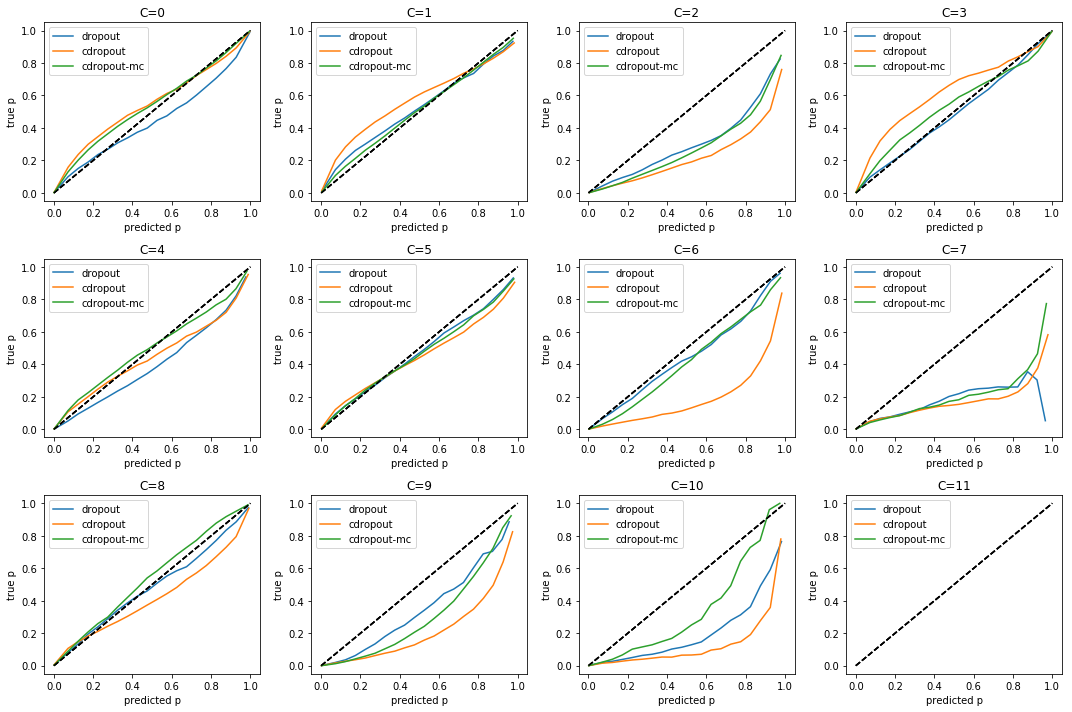
\includegraphics[width=\linewidth]{calibration_plots.png}
\end{subfigure}%
\begin{subfigure}{.5\textwidth}
  \centering
  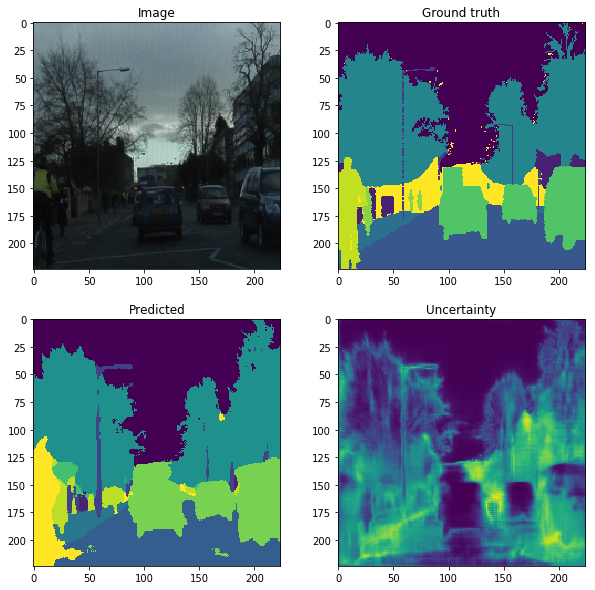
\includegraphics[width=0.7\linewidth]{preview_results.png}
\end{subfigure}
\caption{Calibration plots for 12 classes (a) and example of segmentation and uncertainty (b).}
\label{fig:calib_ex}
\end{figure}

\begin{figure}[!h]
\centering
\centering
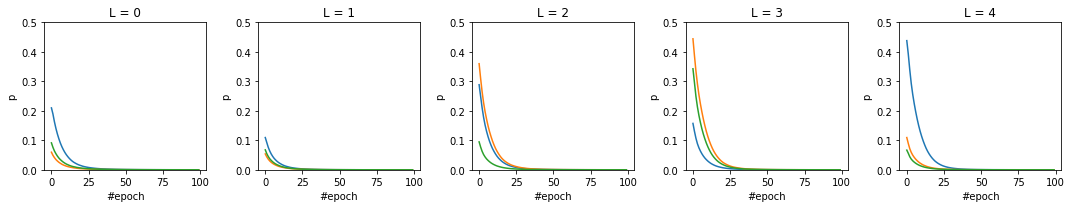
\includegraphics[width=\linewidth]{nlp_probs.png}
\caption{Grapheme-to-Phoneme: dropout rate convergence.}
\label{fig:nlpprobs}
\end{figure}

\begin{figure}[!h]
\centering
\centering
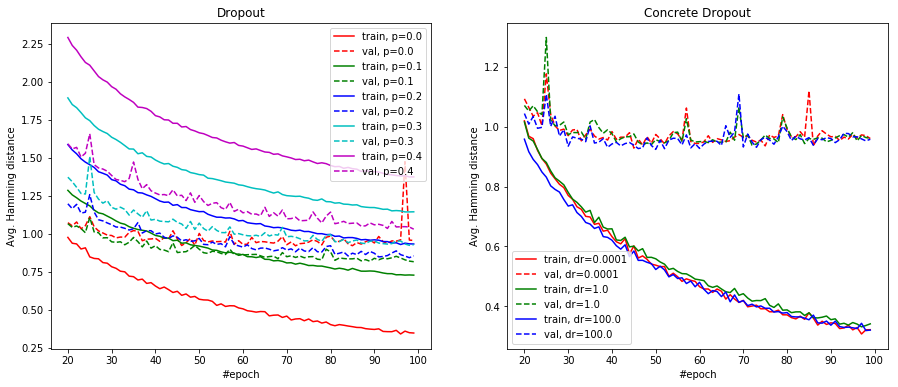
\includegraphics[width=\linewidth]{nlp_curves.png}
\caption{Grapheme-to-Phoneme: learning curves.}
\label{fig:nlpcurves}
\end{figure}

\begin{figure}[!h]
\centering
\begin{subfigure}{.7\textwidth}
  \centering
  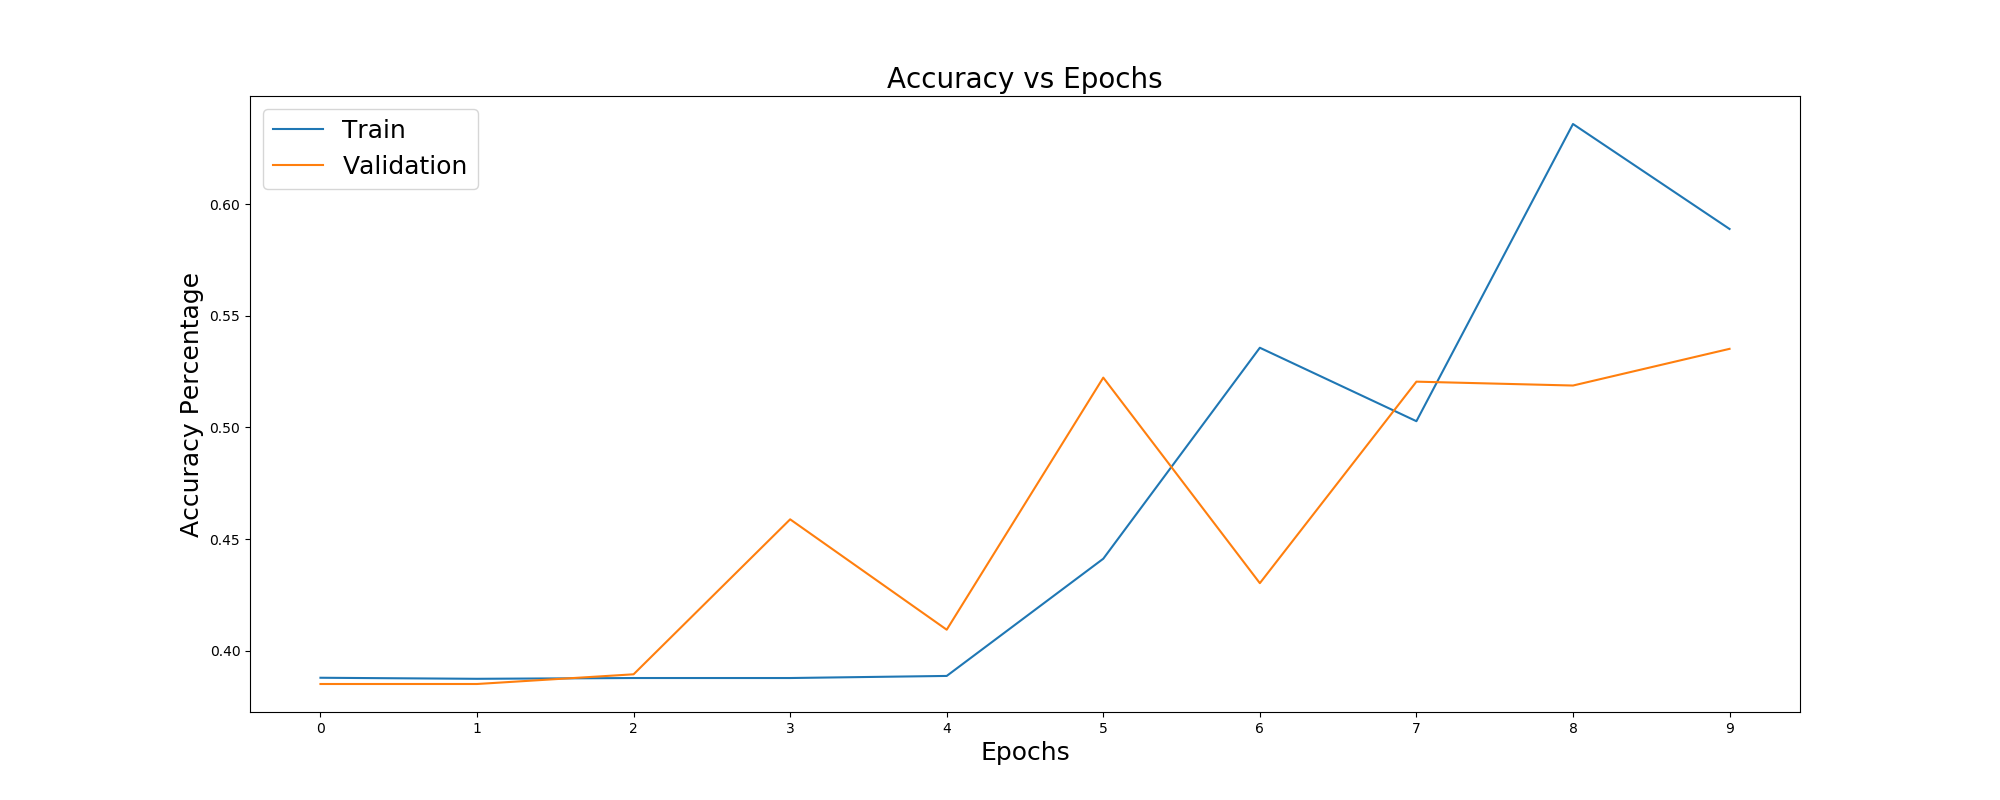
\includegraphics[width=\linewidth]{NLP2_Accuracy_2.png}
  \caption{}
\end{subfigure}%

\begin{subfigure}{.7\textwidth}
  \centering
  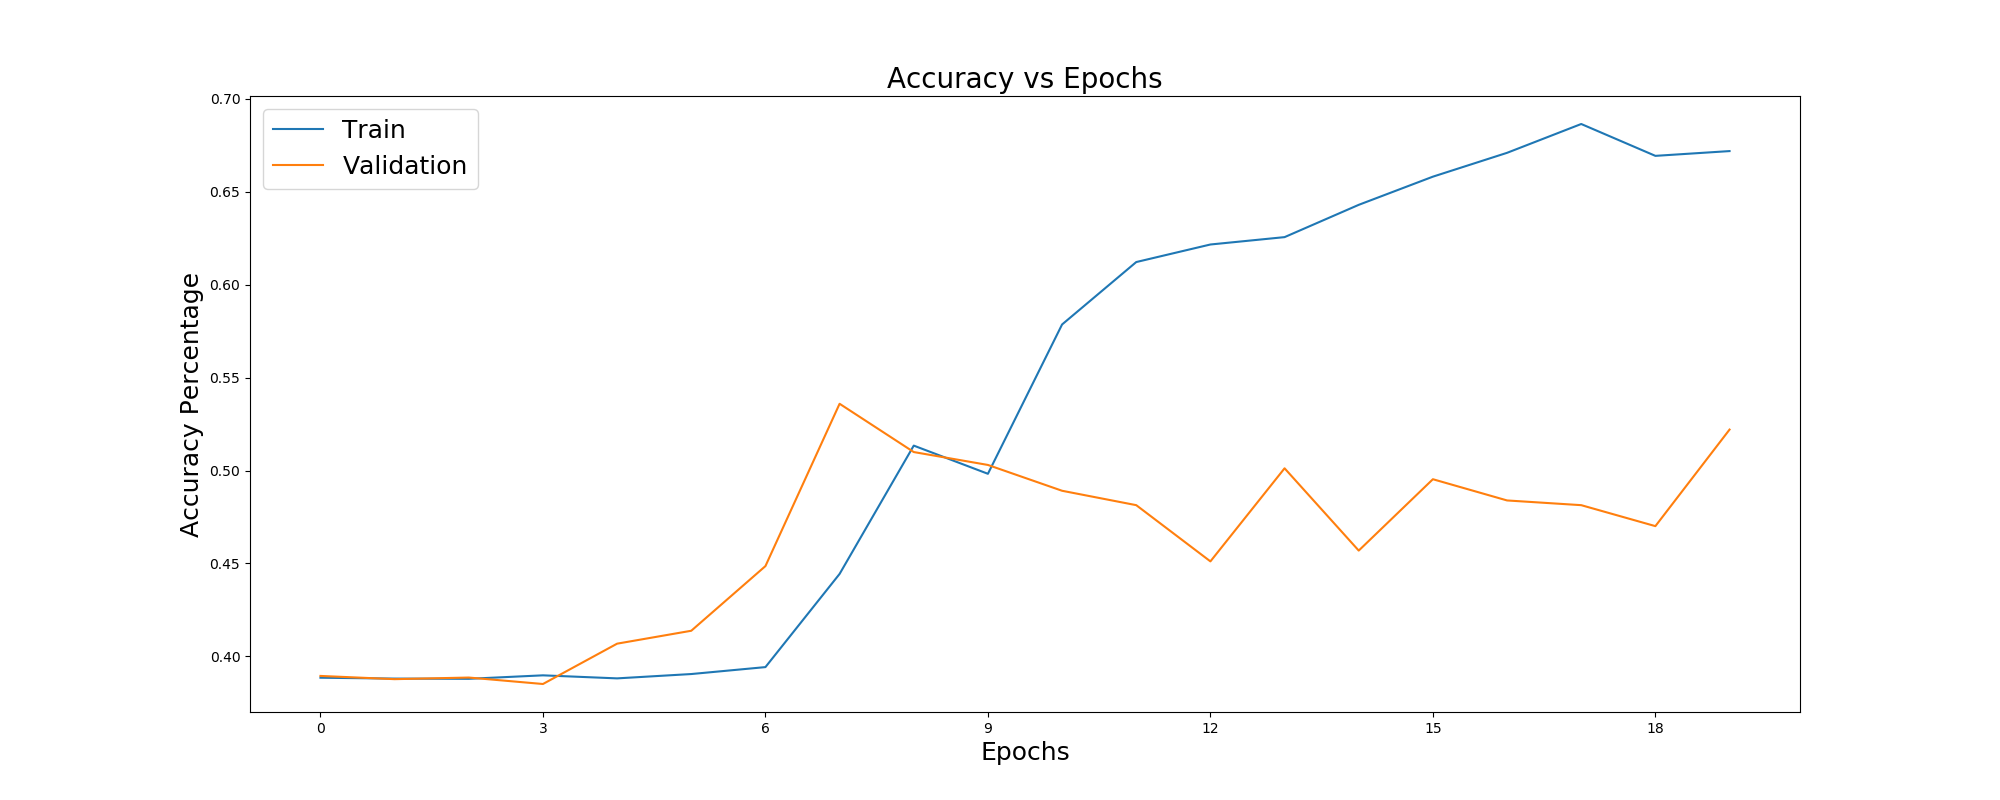
\includegraphics[width=\linewidth]{NLP2_Accuracy_3.png}
  \caption{}
\end{subfigure}%
\caption{(a) Sentiment Classification learning curve for constant dropout (0.5). (b) Sentiment Classification learning curve for concrete dropout.}
\label{fig:sentiment}
\end{figure}

\end{document}
